\documentclass[11pt,a4paper]{article}
\usepackage[T1]{fontenc}
\usepackage[utf8]{inputenc}
\usepackage{newtxtext}
\usepackage[scaled=0.88]{beramono}
\usepackage[margin=24mm,headheight=15pt]{geometry}
\usepackage{amsmath,amsthm,mathtools}
\usepackage{newtxmath}
\usepackage{microtype,bm}
\usepackage{booktabs,tabularx,longtable,array}
\usepackage{enumitem,xcolor,listings}
\usepackage[most]{tcolorbox}
\usepackage{tikz}
\usetikzlibrary{arrows.meta,positioning,calc}
\usepackage{fancyhdr,titlesec}
\usepackage[colorlinks=true,linkcolor=inkblue,citecolor=inkblue,urlcolor=inkblue,breaklinks=true]{hyperref}
\usepackage{bookmark}
\urlstyle{same}
\definecolor{inkblue}{HTML}{214860}
\definecolor{papergray}{HTML}{F5F7F8}
\definecolor{rulegray}{HTML}{D9E0E4}
\titleformat{\section}{\Large\bfseries\color{inkblue}}{\thesection}{0.7em}{}
\titleformat{\subsection}{\large\bfseries}{\thesubsection}{0.7em}{}
\titlespacing*{\section}{0pt}{2.2ex plus .6ex}{1.1ex}
\titlespacing*{\subsection}{0pt}{1.8ex plus .4ex}{0.8ex}
\setlength{\parindent}{0pt}
\setlength{\parskip}{5.5pt plus 1pt}
\setlength{\emergencystretch}{2em}
\setcounter{tocdepth}{2}
\setlist{topsep=3pt,itemsep=2pt,parsep=0pt,leftmargin=1.6em}
\renewcommand{\arraystretch}{1.15}
\newcolumntype{Y}{>{\raggedright\arraybackslash}X}
\newcommand{\dd}{\,\mathrm{d}}
\newcommand{\R}{\mathbb R}
\newcommand{\E}{\mathbb E}
\newcommand{\norm}[1]{\left\lVert#1\right\rVert}
\newcommand{\abs}[1]{\left\lvert#1\right\rvert}
\DeclareMathOperator{\diag}{diag}
\DeclareMathOperator{\proj}{Proj}
\DeclareMathOperator{\clip}{clip}
\DeclareMathOperator*{\argmin}{arg\,min}
\DeclareMathOperator*{\argmax}{arg\,max}
\newtheorem{proposition}{Proposition}[section]
\newtheorem{theorem}[proposition]{Theorem}
\theoremstyle{definition}
\newtheorem{example}[proposition]{Example}
\theoremstyle{remark}
\newtheorem{remark}[proposition]{Remark}
\newtcolorbox{keyidea}[1]{colback=papergray,colframe=rulegray,
  boxrule=0.5pt,arc=1mm,left=8pt,right=8pt,top=6pt,bottom=6pt,
  breakable,title={#1},fonttitle=\bfseries,coltitle=inkblue,colbacktitle=papergray}
\lstdefinestyle{python}{language=Python,basicstyle=\ttfamily\small,
  keywordstyle=\bfseries\color{inkblue},commentstyle=\itshape\color{black!65},
  stringstyle=\color{black!80},showstringspaces=false,columns=fullflexible,
  keepspaces=true,breaklines=true,breakatwhitespace=false,tabsize=4,
  backgroundcolor=\color{papergray},frame=single,rulecolor=\color{rulegray},
  framerule=0.4pt,framesep=6pt,xleftmargin=7pt,xrightmargin=7pt,
  aboveskip=8pt,belowskip=8pt}
\lstset{style=python}
\pagestyle{fancy}
\fancyhf{}
\renewcommand{\headrulewidth}{0.3pt}
\fancyfoot[C]{\small\thepage}
\fancypagestyle{plain}{\fancyhf{}\fancyfoot[C]{\small\thepage}\renewcommand{\headrulewidth}{0pt}}

\hypersetup{pdftitle={Physics-Informed Learning for Cyber Dynamics and Control},pdfauthor={Lu-Xing Yang},pdfsubject={Sparse observations, parameter inference, structured mechanisms, and constrained neural control}}
\fancyhead[L]{\small\sffamily Note 2: PINN and PIDL}
\fancyhead[R]{\small\sffamily Cyber dynamics and decision making}
\begin{document}
\thispagestyle{plain}
{\color{inkblue}\sffamily\small CYBER DYNAMICS AND DECISION MAKING}\par
\vspace{1.0cm}
{\huge\bfseries Physics-Informed Learning for Cyber Dynamics and Control}\par
\vspace{0.35cm}
{\Large Sparse observations, parameter inference, structured mechanisms, and constrained neural control}\par
\vspace{0.45cm}
{\large Lu-Xing Yang}\par
\vspace{0.7cm}
This note develops physics-informed neural networks and model-and-data learning for cyber propagation. It follows one complete inverse-SIR experiment before extending to control, PMP residuals, learned transmission mechanisms, network inference and hybrid events. Derivatives, constraints, observation masks and independent ODE replay are derived explicitly so that each implemented loss has a clear mathematical meaning. The worked examples use the same state and decision semantics as the companion control and learning notes. Prerequisites are elementary ODEs, multivariable calculus, linear algebra and basic Python/PyTorch.
\vspace{0.5cm}
\begin{keyidea}{How to use this note}
Read the model and the mathematical derivation before changing the code. Run the first example, inspect its state and decision curves, and then use the worked extensions. The equations, assumptions and interpretation are included here; the repository supplies the executable implementations.
\end{keyidea}
\clearpage
\begingroup\setlength{\parskip}{0pt}\footnotesize\linespread{0.90}\selectfont\tableofcontents\endgroup
\clearpage

\section{What is unknown, and what information is available?}
Physics-informed learning combines observations with equations that express a proposed mechanism. Its role depends on the unknown object. A forward PINN approximates a trajectory for a known model. An inverse PINN estimates parameters and latent states. A control PINN represents a decision schedule. A PMP-informed method also represents costates and enforces necessary optimality conditions. PIDL is a broader label for learning that uses physical structure, including learned corrections and differentiable simulation \cite{raissi,karniadakis}.

The modeling chain is
\begin{center}
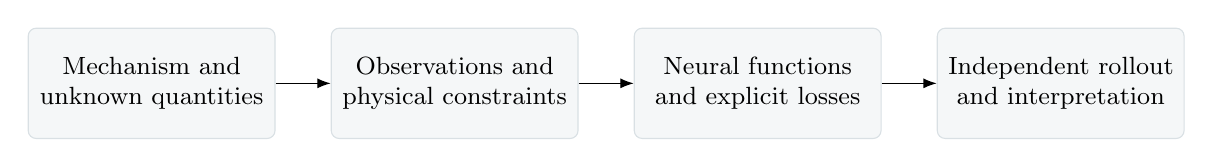
\begin{tikzpicture}[>=Latex,node distance=7mm,
b/.style={draw=rulegray,fill=papergray,rounded corners=1mm,text width=29mm,align=center,minimum height=14mm,font=\small}]
\node[b](a){Mechanism and\\unknown quantities};
\node[b,right=of a](b){Observations and\\physical constraints};
\node[b,right=of b](c){Neural functions\\and explicit losses};
\node[b,right=of c](d){Independent rollout\\and interpretation};
\draw[->](a)--(b);\draw[->](b)--(c);\draw[->](c)--(d);
\end{tikzpicture}
\end{center}
The same chain applies to malware, APT and misinformation models. State meanings and intervention effects are defined before selecting the neural architecture.


\subsection{Why these inference questions arise in cyber control}
The cyber models underlying this tutorial series come from a research line spanning APT security evaluation, patch/repair games and backup/recovery \cite{security2017,patch2018,repair2019,backup2021}, opinion competition and rumor refutation \cite{opinions2020,rumor2021}, and continuous--impulsive interventions \cite{impulse2023,outsource2024,war2024}. These models specify physical states, transition mechanisms and decision objectives. In an inverse problem, some of those states or coefficients are unavailable and must instead be inferred from observations.

The awareness-based propaganda and coupled malware--opinion papers make this motivation especially concrete: behavioral states and network coupling influence propagation, while interventions act through different physical channels \cite{awareness2025,malware2025}. The feedback-loop malware-control study explicitly connects parameter learning with MPC \cite{feedback2024}. This note develops PINN/PIDL tools that can be used to study related inference or control questions. It does not attribute PINN algorithms to those publications: their original model/control contributions and the neural extensions described here are identified separately.

\subsection{Task, output and implementation}
\par\noindent\begin{tabularx}{\linewidth}{@{}p{0.22\linewidth}p{0.29\linewidth}Y@{}}
\toprule
Task & Learned object & Repository route \\
\midrule
Inverse SIR & $x(t)$ and positive rates & \texttt{inverse.py}; the default example. \\
Missing mechanism & $x(t)$, rates and an additional flux & \texttt{pidl.py}. \\
Direct control & $x(t)$ and bounded $u(t)$ & \texttt{control.py}. \\
PMP-informed control & $x(t),u(t),\lambda(t)$ & \texttt{pmp.py}. \\
Node-level inference & Node states and selected heterogeneous parameters & \path{node_problem.py}, \path{node_inverse.py}. \\
Feedback HJB/game values & $V(t,x)$ or player-specific $V_i(t,x)$ & A mathematical extension, not the default executable experiment. \\
\bottomrule
\end{tabularx}\par

\subsection{Install and run}
Inside \texttt{note2-pinn-pidl-cyber-control}, use a separate environment:
\begin{lstlisting}[language={}]
python -m venv .venv
# macOS / Linux:
source .venv/bin/activate
# Windows PowerShell instead:
# .venv\Scripts\Activate.ps1
python -m pip install -e .
python -m cyberpinn
\end{lstlisting}
Use Python 3.11 or 3.12 and install Git for the pinned shared-library dependency. The first experiment runs on a CPU and generates its own observations. It compares a PINN trajectory, an ODE rollout using the PINN's learned rates, and a direct ODE least-squares fit to the same data. No GPU, external dataset or LaTeX installation is needed for this experiment.

The default uses 24 observations, 64 collocation points, a two-hidden-layer width-32 state network, 1,500 Adam steps, and seed 1. These are inspectable teaching settings. The wider study has its own profiles and is invoked separately after the first example is understood.

\section{Mechanistic models and observation maps}
\subsection{The SIR model used for parameter learning}
The first inverse problem is
\begin{align}
\dot S&=-\beta SI, & \dot I&=\beta SI-\gamma I, & \dot R&=\gamma I,
\label{eq:inverse-sir}
\end{align}
with known initial state $(0.95,0.05,0)$ and unknown positive rates $\beta,\gamma$. Time is measured in a chosen unit; both rates have inverse-time units. Synthetic truth uses $\beta=0.8$, $\gamma=0.2$ on $[0,20]$. The values illustrate the procedure and are not fitted measurements of malware incidents.

The physical state is nonnegative and sums to one. Each infection flux $\beta SI$ leaves $S$ and enters $I$; each recovery flux $\gamma I$ leaves $I$ and enters $R$. The vector field is inward-pointing at each nonnegativity boundary. These are properties of the model to preserve when adding controls or learned mechanisms.

\subsection{Measurements are not latent-state truth}
Write the observation equation explicitly:
\begin{equation}
y_j=h(x(t_j),\theta)+\varepsilon_j.
\label{eq:observation}
\end{equation}
For infection fractions, $h(x)=I$. For expected counts in a population of size $n$, $h(x)=nI$. A count observation may need a count likelihood rather than squared error in unscaled proportions. Known initial conditions, known controls, observed compartments and unknown parameters should be stated separately.

The function \texttt{observation\_data} returns the full time grid, clean synthetic truth, observed indices and measured infection values as separate objects. A local seeded generator adds noise only to the observations. Both the PINN and the ODE baseline receive those same values. Noise does not alter the clean latent states used for evaluation. The additive Gaussian measurement example permits noisy values outside $[0,1]$; another measurement process can use an appropriate bounded or count model.

For partial multivariate data, let $M_{jc}$ indicate whether component $c$ is observed at time $t_j$. A masked squared error is
\begin{equation}
\mathcal L_{\rm data}=
\frac{\sum_{j,c}M_{jc}[\hat x_c(t_j)-y_{jc}]^2}{\sum_{j,c}M_{jc}}.
\end{equation}
Missing values contribute no term. Replacing them with zeros and treating those zeros as observations changes the inference problem.

\subsection{Other cyber mechanisms retain the same workflow}
An APT model with vulnerable, compromised, detected and protected states is
\begin{align}
\dot V&=-\beta VC-u_pV+\omega P, &
\dot C&=\beta VC-(\alpha+u_m)C,\nonumber\\
\dot D&=(\alpha+u_m)C-u_rD, &
\dot P&=u_pV+u_rD-\omega P.
\end{align}
Patching, monitoring and repair operate on different transitions. An inverse task might estimate $\beta$ and $\alpha$ from partial detection records; a control task might optimize $u_p,u_m,u_r$ with the rates fixed. Both use the same physical state, but different trainable objects and objectives.

A misinformation model can separate unaware users, misinformation spreaders, counter-message spreaders and inactive users. Counter-messaging may change transmission/conversion rates or cause a campaign reset. The observation map then describes what a dataset actually records---posts, accounts, aggregate prevalence or sampled attitudes---rather than assuming that the complete mathematical state is observed.

\section{Represent functions and constraints in a neural model}
\subsection{The state network and time scaling}
An MLP approximates a function through compositions of affine maps and nonlinear activations. A trajectory network takes time as input and produces state logits. In the inverse SIR implementation,
\begin{equation}
\hat x(t)=\operatorname{softmax}(N_\phi(t/10-1)),
\qquad t\in[0,20].
\end{equation}
The softmax acts across the three compartments at each time. It enforces sum-to-one and positive outputs for finite logits. The known initial $R(0)=0$ is therefore approached through an initial-condition loss, rather than attained exactly by a finite softmax logit.

For $\tau=t/T$, the chain rule is
$\dd\hat x/\dd t=T^{-1}\dd\hat x/\dd\tau$.
For $\tau=2t/T-1$, it is
\begin{equation}
\frac{\dd\hat x}{\dd t}=\frac{2}{T}\frac{\dd\hat x}{\dd\tau}.
\label{eq:time-scale}
\end{equation}
In the supplied inverse network, scaling occurs inside \texttt{forward}, while differentiation is requested with respect to physical $t$. Autograd therefore supplies the scale factor automatically. If the independent differentiable input is already $\tau$, the factor must be supplied explicitly. The two conventions should not be mixed.

\subsection{Hard initial conditions and physical state constraints}
The ansatz $\hat x(t)=x_0+tN_\phi(t)$ enforces $\hat x(0)=x_0$, but imposes neither conservation nor nonnegativity. Applying a softmax afterward changes the initial value in general. A simplex-preserving alternative on $t\ge0$ is
\begin{equation}
\hat x(t)=e^{-ct}x_0+(1-e^{-ct})\operatorname{softmax}(N_\phi(t)),\qquad c>0.
\end{equation}
It enforces the initial state and simplex membership, but also structures the initial derivative and may restrict approximation for a fixed $c$. The first example uses the simpler soft initial-condition loss, keeping this modeling choice visible.

\subsection{Parameter, control and costate outputs}
Positive rate parameters can use
\begin{equation}
\hat\beta=\operatorname{softplus}(b_\beta)+\epsilon,
\qquad \operatorname{softplus}(z)=\log(1+e^z).
\end{equation}
This guarantees positivity, not a known upper bound or identifiability. A specified finite interval can instead use a scaled sigmoid. Those bounds are assumptions that should have an application-specific justification.

A control network $N_u(t)$ represents an open-loop schedule. A policy $\pi(t,x)$ represents feedback only if it is trained and assessed over the relevant state domain. A family of time schedules indexed by an initial state is also not automatically a policy reacting to new measurements. Costates can have either sign and generally require an unconstrained output, rather than softmax or sigmoid.

\subsection{Differentiate each output component}
For a batch of independent time inputs and a pointwise MLP, the derivative array should have the same shape as the predicted states:
\begin{lstlisting}[caption={Componentwise physical-time derivatives}]
import torch

def time_derivative(values, time):
    columns = []
    for j in range(values.shape[1]):
        derivative = torch.autograd.grad(
            values[:, j].sum(), time, create_graph=True
        )[0]
        columns.append(derivative)
    return torch.cat(columns, dim=1)
\end{lstlisting}
Using \texttt{autograd.grad(values.sum(), time)} differentiates the sum of all components. For simplex states that sum is one, so the result can be zero even when every compartment is changing. The componentwise construction avoids this cancellation. The batch-sum shortcut assumes independent samples; a network that couples different batch rows requires more careful Jacobian handling \cite{torchgrad}.

\texttt{create\_graph=True} allows the subsequent residual loss to train the network through these derivatives. Detaching the derivative or the Hamiltonian partials would remove that learning path. Leaf collocation-input gradients can be reset with \texttt{t.grad = None} between iterations; resetting model parameter gradients alone does not clear them.

\section{Forward and inverse PINN losses}
\subsection{Write the residual before writing the optimizer}
For a known control and parameter vector, define
\begin{equation}
r_x(t)=\dot{\hat x}(t)-f(\hat x(t),u(t),\theta,t).
\end{equation}
For inverse SIR, the three residuals are
\begin{align}
r_S&=\dot{\hat S}+\hat\beta\hat S\hat I,\nonumber\\
r_I&=\dot{\hat I}-\hat\beta\hat S\hat I+\hat\gamma\hat I,\label{eq:sir-residual}\\
r_R&=\dot{\hat R}-\hat\gamma\hat I.\nonumber
\end{align}
Let $\operatorname{MSE}$ mean the average of squared entries in its entire argument. Then the actual loss structure is
\begin{equation}
\mathcal L=\operatorname{MSE}(\hat I(t_j^d)-y_j)
+w_0\operatorname{MSE}(\hat x(0)-x_0)
+w_f\operatorname{MSE}(r_x(t_j^f)).
\label{eq:inverse-loss}
\end{equation}
A mean over both time and state components differs by a dimension factor from a mean over time of squared vector norms. Keep the convention fixed when copying loss weights. The default inverse example uses $w_0=10$ and $w_f=1$.

Observation points $t_j^d$ carry measured information. Collocation points $t_j^f$ enforce the assumed equations without adding measured data. For a forward problem, parameters are fixed and the data term may be absent. For an inverse problem, both network weights and selected physical parameters are optimized.

\subsection{One training iteration in the repository}
\begin{lstlisting}[caption={The inverse learning loop in conceptual form}]
optimizer.zero_grad()
t_f.grad = None
beta, gamma = positive(beta_raw), positive(gamma_raw)
loss_data = ((state_net(t_data)[:, 1:2] - I_data) ** 2).mean()
loss_ic = ((state_net(t_zero) - x0) ** 2).mean()
x = state_net(t_f)
r = time_derivative(x, t_f) - sir_rhs(x, beta, gamma)
loss_ode = (r ** 2).mean()
loss = loss_data + w_ic * loss_ic + w_ode * loss_ode
loss.backward()
optimizer.step()
\end{lstlisting}
The trained parameters are represented by unconstrained raw scalars and transformed within the live graph. The state network uses the same physical RHS as the data-generation model in the matched synthetic experiment. The saved inverse history records rate estimates after the logged optimizer update; its loss values are those used to compute that update.

\subsection{Scale losses and sample time deliberately}
State fractions, rates, time derivatives and objectives have different units. Nondimensionalization or physically motivated scale factors can make their losses comparable. If observation components have known noise scales, weighting by those scales is often more meaningful than balancing arbitrary raw magnitudes. A high weight encourages a residual to be small at sampled points; it is not an exact equation constraint.

Uniform collocation is easy to follow. Fresh validation times show whether a low training residual extends between those samples. Sharp changes may require denser samples, adaptive placement or interval decomposition. Training can start with a simple forward task, then a small inverse problem, and then control or game residuals. Adam and optional L-BFGS are numerical choices rather than universal guarantees \cite{wang,krishnapriyan}. The default example uses a bounded Adam run rather than an automatically expanding training schedule.

\section{The first experiment: fit, replay and compare}
\subsection{Use an ordinary ODE fit as a reference}
When only a few parameters of a known ODE are unknown, direct ODE fitting is a meaningful baseline. The code estimates positive rates through their logarithms:
\begin{equation}
\min_{\eta_\beta,\eta_\gamma}\sum_j
\left[I_{\rm ODE}(t_j;e^{\eta_\beta},e^{\eta_\gamma})-y_j\right]^2.
\end{equation}
\texttt{fit\_ode} uses SciPy \texttt{least\_squares} and \texttt{solve\_ivp}, the same observed times/values and the same initial state. The teaching rate bounds are $[0.01,3]$ for both rates. These bounds should be reconsidered for another application, and they differ from the PINN's positive-but-unbounded softplus parameterization.

The ODE solver propagates the specified mechanism. A neural trajectory is an independently optimized function encouraged to satisfy that mechanism. To compare the two meanings, the example also integrates the ODE using the PINN's estimated $(\hat\beta,\hat\gamma)$. Agreement of that replay with the neural trajectory is informative about physical consistency; their disagreement points to a question about training accuracy, information or model assumptions.

\subsection{Inspect the six outputs}
The output directory is \path{results/}. Its two figures are \path{fit.png} and \path{learning.png}. The accompanying tables are \path{observations.csv}, \path{trajectories.csv}, \path{comparison.csv} and \path{training.csv}. The fit plot contains clean truth, measured infection values, the neural trajectory, PINN-rate ODE replay and ODE least squares. The loss plot separates unweighted data, physical and initial-condition terms.

The comparison table reports estimated rates, error against the measured values, and error against clean synthetic infection at unobserved grid times. These held-out times lie \emph{inside} the fitted interval; the physics collocation still spans that interval. The metric tests interpolation, not future forecasting. For a forecasting study, fit observations and collocation only on the declared training interval, and specify how the model is propagated beyond it.

\begin{lstlisting}[language={}]
python -m cyberpinn --iters 3000 --observations 20 --noise 0.01 --seed 4 --output-dir results/noisy
\end{lstlisting}
Changing the number of steps changes optimization effort. Changing observations, noise or the mechanism changes the inference problem. Use the same observed data for each compared method and distinguish uncertainty across training seeds from uncertainty in the measurements.

\subsection{Identifiability is an information question}
In early SIR growth with $S(t)\approx S_0$, the infected state approximately satisfies
\begin{equation}
\dot I\approx(\beta S_0-\gamma)I.
\end{equation}
A short early-time infection curve therefore primarily informs the combination $\beta S_0-\gamma$. More informative times, known interventions, additional observed components or prior information can help separate rates. A small residual alone does not supply the missing distinction.

Structural identifiability asks whether ideal observations uniquely determine a parameter within the model. Practical identifiability concerns the actual noisy, finite observation set. Multiple initial guesses, data windows and sensitivity analyses investigate different aspects of that question. A stable optimizer outcome may still reflect a strong prior or parameterization. With no informative data and unknown parameters, one can compute scenarios consistent with assumptions; unique empirical recovery requires additional information.

\section{Neural optimal control}
\subsection{Distinguish a decision variable from a physical parameter}
After identifying a model, hold its chosen parameters fixed and ask which control minimizes
\begin{equation}
J(u)=\int_0^T L(x,u,t)\dd t+\Phi(x(T)),\qquad
\dot x=f(x,u,t),\quad x(0)=x_0.
\end{equation}
For SIR patching,
\begin{align}
\dot S&=-\beta SI-uS, &
\dot I&=\beta SI-\gamma I, &
\dot R&=\gamma I+uS,
\label{eq:controlled-sir}
\end{align}
with $0\le u\le\bar u$, and
\begin{equation}
L=qI+\frac{b}{2}u^2,\qquad \Phi=q_TI(T),\qquad b>0.
\label{eq:control-objective}
\end{equation}
This control protects susceptible mass. Recovery control would act on infected mass and would give a different optimality formula. Jointly learning poorly identified parameters and an intervention can confound estimation with decision design; a staged identification--control formulation makes the distinction visible.

\subsection{Direct neural control}
A state network $\hat x(t)$ and a bounded schedule network $\hat u(t)$ can be trained using
\begin{equation}
\mathcal L_{\rm direct}=w_J\widehat J+w_f\operatorname{MSE}(\dot{\hat x}-f(\hat x,\hat u))
+w_0\operatorname{MSE}(\hat x(0)-x_0).
\end{equation}
For an equally spaced grid, use an appropriate quadrature for the integral in $\widehat J$; for uniformly sampled times a Monte Carlo estimate is $T$ times the sample mean of the running cost. The horizon factor is essential when balancing running and terminal cost. Nonuniform sampling needs corresponding weights.

Finite loss weights permit tradeoffs between objective reduction and imperfect dynamics. Evaluate the learned control by an independent ODE rollout $x_{\hat u}$ and compute
\begin{equation}
J_{\rm replay}(\hat u)=\int_0^T L(x_{\hat u}(t),\hat u(t),t)\dd t+\Phi(x_{\hat u}(T)).
\label{eq:replay-objective}
\end{equation}
This is the physical objective of the proposed schedule. Computing cost only on an inaccurate neural state curve can underestimate the cost of applying that schedule.

\subsection{PMP-informed control derives a different loss}
Define $H=L+\lambda^\top f$. For the normal minimization problem with a free terminal state,
\begin{equation}
\dot x=f,\qquad \dot\lambda=-H_x,\qquad
\lambda(T)=\Phi_x(x(T)),\qquad
u\in\argmin_{v\in[0,\bar u]}H(x,v,\lambda,t).
\label{eq:pmp}
\end{equation}
These necessary conditions motivate state, costate and control networks. They are distinct from a direct cost-penalty formulation, and do not by themselves prove global optimality \cite{lenhart,liberzon}.

For \eqref{eq:controlled-sir}--\eqref{eq:control-objective},
\begin{align}
H={}&qI+\frac{b}{2}u^2+\lambda_S(-\beta SI-uS)
+\lambda_I(\beta SI-\gamma I)+\lambda_R(\gamma I+uS),\nonumber\\
\dot\lambda_S={}&\beta I(\lambda_S-\lambda_I)+u(\lambda_S-\lambda_R),\nonumber\\
\dot\lambda_I={}&-q+\beta S(\lambda_S-\lambda_I)+\gamma(\lambda_I-\lambda_R),\label{eq:sir-costate}\\
\dot\lambda_R={}&0,\qquad \lambda(T)=(0,q_T,0)^\top.\nonumber
\end{align}
The unconstrained Hamiltonian minimizer is $S(\lambda_S-\lambda_R)/b$. Under the control interval,
\begin{equation}
u_H=\clip\left(\frac{S(\lambda_S-\lambda_R)}{b},0,\bar u\right).
\label{eq:pmp-control}
\end{equation}
Since $H_{uu}=b>0$, this is its exact pointwise minimizer.

\subsection{The correct residual at a control bound}
The first-order condition on the interval is
\begin{equation}
H_u=0\text{ if }0<u<\bar u,\quad
H_u\ge0\text{ if }u=0,\quad
H_u\le0\text{ if }u=\bar u.
\end{equation}
A single projected residual covers all three cases:
\begin{equation}
r_u=u-\proj_{[0,\bar u]}(u-H_u/b)=u-u_H.
\label{eq:projected-pmp}
\end{equation}
For example, $H(u)=u^2/2+2u$ is minimized at $u=0$ on $[0,1]$, although $H_u(0)=2$. The projected residual is zero there; a raw $H_u^2$ penalty is not.

The PMP loss uses
\begin{align}
r_x&=\dot{\hat x}-f(\hat x,\hat u), &
r_\lambda&=\dot{\hat\lambda}+H_x(\hat x,\hat u,\hat\lambda),\nonumber\\
\mathcal L_{\rm PMP}&=w_x\operatorname{MSE}(r_x)+w_\lambda\operatorname{MSE}(r_\lambda)
+w_u\operatorname{MSE}(r_u)+w_b\mathcal L_{\rm boundary},\label{eq:pmp-loss}
\end{align}
where $\mathcal L_{\rm boundary}$ includes the initial state and terminal costate. The \texttt{pmp.py} implementation uses \texttt{projected\_control\_residual}; its coefficient \texttt{B} is $b$ and its state-cost coefficient \texttt{A} is $q$.

\begin{lstlisting}[caption={The bounded Hamiltonian condition used in training}]
H = hamiltonian(x, u, lam, A, B, beta, gamma)
Hx = torch.autograd.grad(H.sum(), x, create_graph=True,
                         retain_graph=True)[0]
Hu = torch.autograd.grad(H.sum(), u, create_graph=True,
                         retain_graph=True)[0]
r_u = u - torch.clamp(u - Hu / B, min=0.0, max=umax)
loss_stationarity = (r_u ** 2).mean()
\end{lstlisting}
The state, costate and control networks are separate functions of time, so these are partial derivatives with respect to their displayed outputs. If a control is analytically substituted as a function of $x$ and $\lambda$, derive the required partials before substitution or account carefully for the computation graph. Differentiating a substituted composite Hamiltonian can introduce unintended chain-rule terms.

For a general differentiable Hamiltonian, $u-\proj_U(u-\eta H_u)$ is a constrained first-order residual for $\eta>0$. A zero residual is a pointwise minimum when the Hamiltonian is convex in $u$; otherwise it is only a stationary candidate. For a nonconvex or discrete action set, use the actual admissible Hamiltonian minimization rather than pretending that interval projection solves it.

\section{What accuracy and optimality can be concluded?}
\subsection{Separate the four outputs of an inverse-control study}
Data agreement concerns the observation map. Trajectory accuracy concerns the whole state. Parameter recovery concerns the unknown coefficients. Control performance concerns the independently replayed objective. A result can be strong on one of these and weak on another. Choose the comparison that answers the intended scientific question.

For synthetic truth, report state and parameter errors on a separate grid. For real data, true hidden states and rates are usually unavailable; held-out measurements and sensitivity to assumptions then become central. For control, compare replayed state/control curves and cost components under matched constraints and initial states. FBSM, direct transcription, no intervention and informative static/feedback strategies provide different reference points.

\subsection{A residual-to-trajectory estimate}
The following elementary estimate explains why physical residuals are useful, while also showing the assumptions needed to interpret them.
\begin{proposition}[Residual consistency for a fixed known model]
Let $y$ solve $\dot y=f(y,u,t)$ with initial state $y_0$. Let $\hat x$ be differentiable and $r=\dot{\hat x}-f(\hat x,u,t)$. Suppose $f$ is Lipschitz in state with constant $L$ on a domain containing both trajectories. Then
\begin{equation}
\norm{\hat x(t)-y(t)}\le e^{Lt}\norm{\hat x(0)-y_0}
+\int_0^t e^{L(t-s)}\norm{r(s)}\dd s.
\label{eq:residual-bound}
\end{equation}
\end{proposition}
\begin{proof}
Subtract the state equations and use the integral form of the error. Lipschitz continuity bounds the vector-field difference by $L\norm{\hat x-y}$. Gronwall's inequality gives \eqref{eq:residual-bound}.
\end{proof}
The estimate uses the residual throughout the interval, not only its finite training-point average. Long horizons, large $L$, stiff dynamics and missed residual peaks can enlarge error. With uncertain parameters, the difference between $f(\cdot,\hat\theta)$ and $f(\cdot,\theta^*)$ introduces an additional forcing term; small residual under the learned parameters alone does not bound error against an unknown true mechanism.

For a reset with Lipschitz constant $L_G$ and jump residual $r_G=\hat x^+-G(\hat x^-,v)$, the corresponding event error obeys
\begin{equation}
\norm{\hat x^+-y^+}\le L_G\norm{\hat x^--y^-}+\norm{r_G}.
\end{equation}
This connects interval accuracy to event accuracy without forcing a smooth approximation through a jump.

\subsection{Necessary conditions and sufficient verification}
A small PMP loss is evidence about the sampled necessary conditions. Global sufficiency can follow from appropriate joint Hamiltonian/terminal convexity, or from a value-function verification theorem, under their assumptions. Nonlinear SIR dynamics do not automatically satisfy joint convexity merely because the control cost is quadratic.

For a smooth candidate value function in a minimization problem,
\begin{equation}
V_t+\min_u\{L+\nabla V^\top f\}=0,\qquad V(T,x)=\Phi(x)
\end{equation}
provides a different route. Along any admissible trajectory, $L+V_t+\nabla V^\top f\ge0$; equality for a minimizing feedback selector verifies optimality. Residual-based PDE approaches such as DGM and differential-equation libraries such as DeepXDE provide related computational tools \cite{dgm,deepxde}. A neural HJB residual sampled at finitely many state-time points is an approximation to that global statement. The state-domain coverage and approximation error remain part of the assessment.

\section{PIDL: learn a structured missing mechanism}
\subsection{Conservation and positivity are separate properties}
The synthetic PIDL example extends SIR with an extra transmission flux:
\begin{equation}
f_{\rm true}(x)=f_{\rm SIR}(x;\beta,\gamma)
+(-1,1,0)^\top qSI^2,\qquad q\ge0.
\end{equation}
Opposite signs preserve the sum of compartments. But a generic nonnegative correction $g_\phi(x)$ subtracted from $S$ can still make $\dot S<0$ at $S=0$. Conservation alone does not preserve nonnegativity.

Use a nonnegative, state-gated flux,
\begin{equation}
g_\phi(x)=SI\operatorname{softplus}(N_\phi(x)),\qquad
f_{\rm PIDL}=f_{\rm SIR}+(-1,1,0)^\top g_\phi(x).
\label{eq:pidl-flux}
\end{equation}
The extra transmission vanishes at $S=0$ and $I=0$, matching the contact-driven mechanism. At $R=0$, recovery contributes a nonnegative derivative. Thus the physical simplex remains invariant for the continuous model. The correction network returns the \emph{flux} $g_\phi$, not merely the unconstrained rate output.

\begin{lstlisting}[caption={The physical structure is visible in the correction}]
class CorrectionNet(torch.nn.Module):
    def __init__(self, width=64, depth=2):
        super().__init__()
        self.net = MLP(3, 1, width=width, depth=depth)

    def forward(self, x):
        rate = torch.nn.functional.softplus(self.net(x))
        return x[..., 0:1] * x[..., 1:2] * rate
\end{lstlisting}
For a different missing mechanism, derive its source compartment, destination compartment and boundary behavior first. External seeding, for example, need not vanish at $I=0$ and would require a different interpretation. A sign or state gate should express a scientific assumption, not merely improve numerical appearance.

\subsection{A correction is not automatically an identified mechanism}
The code learns positive base rates as well as a flexible correction. In \eqref{eq:pidl-flux}, the total infection flux is $SI[\beta+\operatorname{softplus}(N_\phi(x))]$. A constant contribution can be shifted between the base rate and the neural rate while preserving the total over the observed region. Regularizing the correction selects among explanations; it does not create unique information about their decomposition.

Compare the known-only model with the corrected model on the same observations and held-out trajectories. Examine the total effective flux, parameter sensitivity and behavior under new initial conditions. A small, stable correction can be useful for prediction or control even when its decomposition into a named physical cause is not uniquely identified.

\subsection{PINN and differentiable simulation are complementary}
A PINN represents the trajectory and penalizes its differential residual. A neural ODE or differentiable-simulation model represents a vector field and obtains trajectories by integration \cite{neuralode}. Both can use a structured correction. Their numerical errors and optimization costs differ: collocation residuals assess local equation agreement, while integration propagates a vector field through time. Independent replay remains useful in either case.

\section{Game-aware and hybrid extensions}
\subsection{One state, several objectives and costates}
For a two-player open-loop game with costs $J_i=\Phi_i+\int L_i\dd t$, define
$H_i=L_i+\lambda_i^\top f$. A candidate has one shared state equation and, for each player,
\begin{equation}
\dot\lambda_i=-(H_i)_x,\qquad
\lambda_i(T)=(\Phi_i)_x,\qquad
u_i\in\argmin_{v_i\in U_i}H_i(x,v_i,u_{-i},\lambda_i,t).
\end{equation}
Use the appropriate maximization convention if a player is defined by payoff. For convex action sets, projected residuals can express each player's constrained first-order condition. A scalar sum of residual losses is a numerical device for solving these equations; it is not the sum of players' economic objectives.

A time-only game PINN produces open-loop schedules for the specified initial state. A feedback Nash formulation instead involves player-specific value functions and coupled HJB equations. Neither form is certified merely by a small empirical residual. Frozen-opponent unilateral-response searches provide useful evidence; their attained improvements are lower bounds on global exploitability, unless the best-response problem is solved with a suitable guarantee.

\subsection{Represent both sides of an impulse}
For an event at $\tau$,
\begin{equation}
\dot x=f(x,u,t),\quad t\ne\tau,\qquad x(\tau^+)=G(x(\tau^-),v).
\end{equation}
Use separate interval networks, or a representation explicitly capable of a discontinuity. A single smooth network evaluated at the same time cannot provide two different one-sided values. Define left and right endpoint predictions and include
\begin{equation}
r_G=\hat x^+(\tau)-G(\hat x^-(\tau),v).
\end{equation}
For a continuous--impulsive optimal-control problem, add the costate jump residual
\begin{equation}
r_{\lambda,G}=\hat\lambda^- -G_x^\top\hat\lambda^+-K_x.
\end{equation}
A free interior impulse magnitude satisfies the appropriate first-order condition involving $K_v+G_v^\top\lambda^+$. A freely optimized interior event time additionally has
\begin{equation}
H^- -H^+ +K_t+(\lambda^+)^\top G_t=0
\end{equation}
under the smooth unconstrained-timing assumptions. Guards, active spacing constraints and endpoint events require their own conditions. Fixed event times do not need a free-time residual.

For interval $[\tau_\ell,\tau_{\ell+1}]$, local time $s=(t-\tau_\ell)/h_\ell$, $h_\ell=\tau_{\ell+1}-\tau_\ell$, gives
$\dot x=h_\ell^{-1}\partial_s x$. If event times are trainable, the duration enters both the residual and objective quadrature. Ordered times and any minimum spacing must be enforced by the optimization formulation.

\subsection{A switched rate has a different boundary condition}
A sampled action can change the vector field while the state remains continuous. Then interval networks should match state values at the decision boundary, without an impulse reset residual. The time derivative may have a kink. A mode--intensity action is not by itself evidence of a state jump. For actual impulse decisions, the value-function obstacle in a minimization problem is $\mathcal MV-V\ge0$, consistent with the QVI developed in the foundation note.

\section{Node-level and degree-level inference}
\subsection{Build the network input before the loss}
For node-level propagation, construct $A_{ij}$ so that node $j$ influences node $i$, and preserve node ordering in every state, parameter and observation array. A sparse incoming pressure is
\begin{equation}
p_i(t)=\sum_jA_{ij}b_jI_j(t).
\end{equation}
A heterogeneous node-SIPS model can use $s_iS_ip_i$ as the infection flux, with recovery, protection and intervention efficacies attached to their corresponding transitions. The node state has three compartments per node, whereas the simplest degree SIS state has one infection fraction per degree class. Their tensor dimensions and constraints differ.

For a degree model, calculate $N_k,P(k),\bar k$ from the full input graph. The uncorrelated closure uses $\Theta=\sum_k kP(k)x_k/\bar k$. A network with correlations can use a conditional mixing matrix. Degree is an unweighted neighbor count unless a weighted closure is specifically derived; in-degree alone does not specify a directed mean-field model.

\subsection{Observation masks define the generalization question}
The node-level code separates observed nodes, observed times and held-out combinations. Holding out time on observed nodes tests temporal interpolation or forecasting depending on the split. Holding out nodes at observed times tests spatial reconstruction. Holding out both tests a joint task. Report the actual mask used for each metric; averaging all unobserved entries into one number can obscure their distinct difficulties.

A dense time-to-all-nodes network has an output dimension tied to the chosen graph. A factorized network uses time and node features to generate node predictions with shared weights. Such sharing permits a transfer experiment, but useful transfer still depends on feature meaning, graph distribution and the learned mechanism. Architecture comparisons should state capacity, observations and training effort.

\subsection{Resolve parameter scaling ambiguities explicitly}
If infection contains a product $s_iA_{ij}b_j$, then for $c>0$ the transformation
$s_i\mapsto cs_i$, $b_j\mapsto b_j/c$ leaves that product unchanged. A normalization such as a unit geometric mean for infectivity fixes a representation. It does not add an extra measured quantity or prove that susceptibility and infectivity are individually identifiable from the available data.

This distinction is useful when combining inference with control: predictions may determine an effective transmission operator sufficiently well for a decision even while separate biological/social interpretations remain uncertain. Evaluate the decision using that uncertainty rather than relying on labels alone.

\section{Adapt the implementation through a single sequence}
\subsection{Read the first example before the extensions}
Read \texttt{cli.run\_example}, then \texttt{inverse.observation\_data}, then \texttt{inverse.train}. The first file assembles the same-data comparison and replay. The second defines precisely what is observed. The third expresses the neural approximation and losses. The shared library supplies the MLP, physical RHS and derivative helper rather than duplicating them in every example.

For a new model, align the state ordering, observation map, parameter constraints, physical-time scale, RHS, neural outputs and evaluation solver. When adding control, also derive the objective, Hamiltonian, costate boundary conditions and bounded optimizer. When adding impulses, derive left/right state and costate relations before training. This keeps each loss tied to a mathematical statement.

\subsection{Run a focused extension from Python}
\begin{lstlisting}[caption={Train the bounded PMP example through its existing API}]
from cyberpinn.configs import PMPConfig
from cyberpinn.pmp import train

cfg = PMPConfig(
    iters=500, width=32, depth=2, n_collocation=64,
    device="cpu", log_every=100, seed=4
)
state_net, costate_net, control_net, history = train(cfg)
print(history[-1])
\end{lstlisting}
The call illustrates the interface and an explicitly bounded training budget. Its final control should then be replayed and compared with the same physical model. Increasing the training budget is justified by measured accuracy and decision behavior, rather than by assuming that a longer run must converge.

The existing broader study is available with
\begin{lstlisting}[language={}]
python -m cyberpinn study --device cpu --output-dir results/study
\end{lstlisting}
It has separate method profiles. The default first-example flags do not redefine every method in that preset. The ordinary entry point remains \texttt{python -m cyberpinn}.

\subsection{From inference to feedback decisions}
A practical application can observe the system, estimate latent states/rates, choose a control, apply it, and update from new observations. Each stage has different information and uncertainty. A fitted time-only trajectory does not automatically supply an online estimator, and a fitted time-only control does not automatically supply feedback. The foundation note develops continuous and hybrid decision theory; Note 1 develops sampled policy learning. Their interfaces can be combined once the observation and decision meanings agree.


\section{Use the cyber-control papers to design meaningful inverse problems}
\subsection{State estimation before security evaluation or control}
Yang et al.'s APT security-evaluation model relates dynamical behavior to a security assessment \cite{security2017}. A related inverse study must first specify which of those states are observed and which mechanisms are known. Observing a security score is not the same as observing every compartment or node. Define the observation operator before choosing a network output or residual.

The patch-injection, repair and backup/recovery studies then motivate decision-relevant inference \cite{patch2018,repair2019,backup2021}. For example, uncertainty in recovery capability may matter differently from uncertainty in transmission. The inverse objective should recover the quantities needed by the stated controller, and the final evaluation should replay that controller under a separately specified physical model. Accurate interpolation of observed infection alone does not establish accurate recovery costs or control decisions.

\subsection{Learning a parameter and learning a missing flux are different tasks}
Jafar et al. use learning to estimate unknown parameters in an MPC feedback loop \cite{feedback2024}. This motivates a concrete interface for the PINN example: infer parameters from observations, replay the inferred model, compute an admissible intervention and evaluate the resulting state/cost. Substituting a PINN for the paper's estimator is a new experiment, not an existing result of that paper.

The structured PIDL correction in this note answers a different question: whether a specified mechanistic family omits an additional state-dependent flux. In an awareness-coupled model, an apparent extra infection flux could reflect an unobserved behavioral state rather than a new transmission law \cite{awareness2025,malware2025}. Compare the explicit coupled-state model with an effective correction only after stating what is measured and which parameterizations are distinguishable from those measurements.

\subsection{Two coupled layers and event-conditioned data}
The malware--opinion paper has coupled infection and awareness dynamics and separate patching/training impulse controls \cite{malware2025}. For a proposed inverse extension, let $c(t)$ and $o(t)$ denote those two state vectors and use an observation map selecting the measured nodes, times and components. The actual physical RHS and reset maps must come from the chosen model. The earlier one-state SIR residual cannot represent that coupling merely by adding more output columns.

Data at an intervention time require a left/right convention. A measurement just before patching is an observation of $c(\tau^-)$; one just after is of $c(\tau^+)$. Awareness training can change $o$ while $c$ remains continuous at that same event. Separate interval networks and a reset residual represent these distinctions. This is a suggested PINN formulation for the model class; the cited publication develops its own impulse-control approach.

The awareness-based propaganda study and its no-awareness comparison also motivate an identifiable ablation \cite{awareness2025}: determine whether additional awareness observations improve held-out propagation prediction, rather than using hidden synthetic states during training without declaring them. A model without awareness and a model with unobserved awareness have different statistical meanings.

\subsection{Strategic objectives survive a neural solver}
The conflicting-opinion and rumor-refutation papers provide examples of player-specific objectives \cite{opinions2020,rumor2021}; the propaganda-war paper adds hybrid decisions \cite{war2024}. A neural solver should retain one costate/value representation per player where the formulation requires it. Adding residuals to one training loss does not turn a general-sum game into a common-payoff problem.

Impulsive artificial defense and outsourced defense extend this lesson to events and decision ownership \cite{impulse2023,outsource2024}. A learning-based numerical extension must retain the original continuous/event decision sets, costate jumps and timing constraints. Compare it with the original method on the same mathematical problem before interpreting a difference as improved optimization. Frozen-opponent response tests, independent ODE/event replay and data holdouts answer complementary questions; none replaces the others.

\begin{keyidea}{A connected research workflow}
Choose a published mechanism and its decision question; state the available measurements; identify the unknown quantities; derive the residuals and constraints; compare inference with a matched mechanistic baseline; and evaluate decisions using independent physical replay. This connects the author's model-based research with new learning tools while preserving the meaning of each contribution.
\end{keyidea}

\appendix
\section{A complete ODE-fitting reference}
The following compact example shows the baseline idea using standard SciPy functions. It uses observed infection values only; it does not feed hidden state truth into the fit.
\begin{lstlisting}[caption={Mechanistic fitting with the same observation operator}]
import numpy as np
from scipy.integrate import solve_ivp
from scipy.optimize import least_squares

def trajectory(time, beta, gamma):
    def rhs(t, x):
        S, I, R = x
        infection, recovery = beta * S * I, gamma * I
        return [-infection, infection - recovery, recovery]
    sol = solve_ivp(rhs, (0.0, float(time[-1])),
                    [0.95, 0.05, 0.0], t_eval=time,
                    rtol=1e-8, atol=1e-10)
    if not sol.success:
        raise RuntimeError(sol.message)
    return sol.y.T

# Replace these synthetic observations by a validated data loader.
time = np.linspace(0.0, 20.0, 24)
observed_I = trajectory(time, 0.8, 0.2)[:, 1]
fit = least_squares(
    lambda z: trajectory(time, *np.exp(z))[:, 1] - observed_I,
    np.log([0.7, 0.3]),
    bounds=(np.log([0.01, 0.01]), np.log([3.0, 3.0]))
if not fit.success:
    raise RuntimeError(fit.message)
print("beta, gamma:", np.exp(fit.x))
\end{lstlisting}
For a general dataset, check increasing unique observation times, physical units, the known/estimated initial state and the measurement model. The library solver's tolerances concern numerical integration; the statistical uncertainty of fitted rates is a separate issue \cite{scipy}.

\section{Short exercises with worked answers}
\paragraph{Time scaling.} A network accepts $\tau=2t/T-1$. What is the physical derivative if differentiation is taken with respect to $\tau$?\par
\emph{Answer:} $(2/T)\partial_\tau\hat x$. If scaling is inside a network whose differentiable input remains $t$, the chain rule is already included.

\paragraph{Summed derivatives.} A simplex network has $S+I+R=1$. Why can differentiating the sum return zero?\par
\emph{Answer:} It differentiates the conservation identity. The ODE requires three separate derivatives, which can be nonzero while summing to zero.

\paragraph{Boundary flux.} Does $(-g,+g,0)$ with $g>0$ preserve the physical simplex at $S=0$?\par
\emph{Answer:} It preserves total mass but points out of the nonnegative region because $\dot S=-g<0$. A contact-driven flux $SIh(x)$ with $h\ge0$ vanishes on the appropriate boundaries.

\paragraph{Parameter replay.} A neural curve fits $I(t)$ but its learned rates generate a different ODE curve. Which output is the physical prediction of those rates?\par
\emph{Answer:} The ODE replay. The neural fit is a separate approximation whose residual/initial consistency must be assessed before equating the two.

\paragraph{Optimality at the upper bound.} For a minimization Hamiltonian with $u=\bar u$ and $H_u<0$, should the raw derivative be driven to zero?\par
\emph{Answer:} No. The derivative points toward increasing $u$, which is infeasible. The projected residual is zero at the constrained optimum.

\section{Development and PDF compilation}
\begin{lstlisting}[language={}]
python -m pip install -e ".[dev]"
pytest -q
python -m cyberpinn check
python -m cyberpinn docs
\end{lstlisting}
Only \texttt{docs} requires LaTeX/\texttt{latexmk}. The mathematical tests and small execution checks support implementation correctness; parameter recovery, control quality and equilibrium claims require their corresponding data and comparison evidence.

\clearpage
\begin{thebibliography}{99}
\bibitem{raissi} M. Raissi, P. Perdikaris and G. E. Karniadakis, ``Physics-informed neural networks: A deep learning framework for solving forward and inverse problems involving nonlinear partial differential equations,'' \emph{Journal of Computational Physics}, 378, 686--707, 2019.
\bibitem{karniadakis} G. E. Karniadakis et al., ``Physics-informed machine learning,'' \emph{Nature Reviews Physics}, 3, 422--440, 2021.
\bibitem{torchgrad} PyTorch developers, \emph{torch.autograd.grad}, official documentation. \url{https://docs.pytorch.org/docs/stable/generated/torch.autograd.grad.html}.
\bibitem{wang} S. Wang, Y. Teng and P. Perdikaris, ``Understanding and mitigating gradient flow pathologies in physics-informed neural networks,'' \emph{SIAM Journal on Scientific Computing}, 43(5), A3055--A3081, 2021.
\bibitem{krishnapriyan} A. Krishnapriyan et al., ``Characterizing possible failure modes in physics-informed neural networks,'' \emph{Advances in Neural Information Processing Systems}, 2021.
\bibitem{lenhart} S. Lenhart and J. T. Workman, \emph{Optimal Control Applied to Biological Models}. Chapman and Hall/CRC, 2007.
\bibitem{liberzon} D. Liberzon, \emph{Calculus of Variations and Optimal Control Theory: A Concise Introduction}. Princeton University Press, 2012.
\bibitem{neuralode} R. T. Q. Chen, Y. Rubanova, J. Bettencourt and D. Duvenaud, ``Neural ordinary differential equations,'' \emph{Advances in Neural Information Processing Systems}, 2018.
\bibitem{scipy} SciPy developers, \emph{solve\_ivp} and \emph{least\_squares}, official documentation. \url{https://docs.scipy.org/doc/scipy/reference/integrate.html}; \url{https://docs.scipy.org/doc/scipy/reference/optimize.html}.
\bibitem{deepxde} L. Lu, X. Meng, Z. Mao and G. E. Karniadakis, ``DeepXDE: A deep learning library for solving differential equations,'' \emph{SIAM Review}, 63(1), 208--228, 2021.
\bibitem{dgm} J. Sirignano and K. Spiliopoulos, ``DGM: A deep learning algorithm for solving partial differential equations,'' \emph{Journal of Computational Physics}, 375, 1339--1364, 2018.

\bibitem{security2017} L.-X. Yang, P. Li, X. Yang and Y. Y. Tang, ``Security evaluation of the cyber networks under advanced persistent threats,'' \emph{IEEE Access}, 5, 20111--20123, 2017. \href{https://doi.org/10.1109/ACCESS.2017.2757944}{doi:10.1109/ACCESS.2017.2757944}.

\bibitem{patch2018} L.-X. Yang, P. Li, X. Yang, Y. Xiang and W. Zhou, ``A differential game approach to patch injection,'' \emph{IEEE Access}, 6, 58924--58938, 2018. \href{https://doi.org/10.1109/ACCESS.2018.2874446}{doi:10.1109/ACCESS.2018.2874446}.

\bibitem{repair2019} L.-X. Yang, P. Li, Y. Zhang, X. Yang, Y. Xiang and W. Zhou, ``Effective repair strategy against advanced persistent threat: A differential game approach,'' \emph{IEEE Transactions on Information Forensics and Security}, 14(7), 1713--1728, 2019. \href{https://doi.org/10.1109/TIFS.2018.2885251}{doi:10.1109/TIFS.2018.2885251}.

\bibitem{backup2021} L.-X. Yang, K. Huang, X. Yang, Y. Zhang, Y. Xiang and Y. Y. Tang, ``Defense against advanced persistent threat through data backup and recovery,'' \emph{IEEE Transactions on Network Science and Engineering}, 8(3), 2001--2013, 2021. \href{https://doi.org/10.1109/TNSE.2020.3040247}{doi:10.1109/TNSE.2020.3040247}.

\bibitem{opinions2020} L.-X. Yang, P. Li, X. Yang, Y. Xiang and Y. Y. Tang, ``Simultaneous benefit maximization of conflicting opinions: Modeling and analysis,'' \emph{IEEE Systems Journal}, 14(2), 1623--1634, 2020. \href{https://doi.org/10.1109/JSYST.2020.2964004}{doi:10.1109/JSYST.2020.2964004}.

\bibitem{rumor2021} D.-W. Huang, L.-X. Yang, P. Li, X. Yang and Y. Y. Tang, ``Developing cost-effective rumor-refuting strategy through game-theoretic approach,'' \emph{IEEE Systems Journal}, 15(4), 5034--5045, 2021. \href{https://doi.org/10.1109/JSYST.2020.3020078}{doi:10.1109/JSYST.2020.3020078}.

\bibitem{impulse2023} H. Sun, X. Yang, L.-X. Yang, K. Huang and G. Li, ``Impulsive artificial defense against advanced persistent threat,'' \emph{IEEE Transactions on Information Forensics and Security}, 18, 3506--3516, 2023. \href{https://doi.org/10.1109/TIFS.2023.3284564}{doi:10.1109/TIFS.2023.3284564}.

\bibitem{outsource2024} Y. Qin, X. Yang, L.-X. Yang and K. Huang, ``Modeling and study of defense outsourcing against advanced persistent threat through impulsive differential game approach,'' \emph{Computers \& Security}, 145, 104003, 2024. \href{https://doi.org/10.1016/j.cose.2024.104003}{doi:10.1016/j.cose.2024.104003}.

\bibitem{feedback2024} M. T. Jafar, L.-X. Yang, G. Li, Q. Zhu and C. Gan, ``Minimizing malware propagation in Internet of Things networks: An optimal control using feedback loop approach,'' \emph{IEEE Transactions on Information Forensics and Security}, 19, 9682--9697, 2024. \href{https://doi.org/10.1109/TIFS.2024.3463965}{doi:10.1109/TIFS.2024.3463965}.

\bibitem{war2024} X. Cheng, L.-X. Yang, Q. Zhu, C. Gan, X. Yang and G. Li, ``Cost-effective hybrid control strategies for dynamical propaganda war game,'' \emph{IEEE Transactions on Information Forensics and Security}, 19, 9789--9802, 2024. \href{https://doi.org/10.1109/TIFS.2024.3468903}{doi:10.1109/TIFS.2024.3468903}. Author code: \href{https://github.com/XiaojuanCheng/PropagandaWar_TIFS_2024_Code}{PropagandaWar\_TIFS\_2024\_Code}.

\bibitem{awareness2025} X. Cheng, L.-X. Yang, Q. Zhu, C. Gan and G. Li, ``Impulse strategies for suppressing cyber propaganda with awareness,'' \emph{IEEE Transactions on Computational Social Systems}, 12(5), 2685--2695, 2025. \href{https://doi.org/10.1109/TCSS.2024.3522889}{doi:10.1109/TCSS.2024.3522889}. Author code: \href{https://github.com/XiaojuanCheng/Propaganda_TCSS_2025_Code}{Propaganda\_TCSS\_2025\_Code}.

\bibitem{malware2025} X. Cheng, L.-X. Yang, G. Li, Z. Ma, T. Zhu, L. Wang and S. Duan, ``Modeling and mitigating social engineering malware: Integrating malware-opinion dynamics with optimal impulse control approaches,'' \emph{IEEE Transactions on Information Forensics and Security}, 20, 12231--12244, 2025. \href{https://doi.org/10.1109/TIFS.2025.3630005}{doi:10.1109/TIFS.2025.3630005}. Author code: \href{https://github.com/XiaojuanCheng/OpinionMalware_TIFS_2025_Code}{OpinionMalware\_TIFS\_2025\_Code}.
\end{thebibliography}
\end{document}
